\chapter{Vertex Detectors in Belle II }

In principle, the function of first a few layers of detectors is to perform the precise tracking in order to measure the decay vertices of B mesons. In Belle II experiment, vertex detectors including pixel detectors (PXD) and silicon vertex detectors (SVD) work for this purpose exclusively. Two sections of detectors are isntalled in Belle II orderly to meet the need of the different characteristics of beam and particle environment along with the growth of radius away from IP. 

\begin{table}[hbp]
	\centering
	\caption{VXD Index, 1 and 2 are PXD, 3 \text{-} 6 are SVD}
	\begin{tabular}{c|c|c|c|c|c|c}
		\hline
		Layer & 1 & 2 & 3 & 4 & 5 &6 \\
		\hline
		Radius(mm) & 14 & 22 & 38 & 80 & 104 & 135 \\
		\hline
		Num of Ladders & 8 & 12 & 7 & 10 & 12 & 16 \\
		\hline
	\end{tabular}
\end{table}

\section{Pixel Detector (PXD)}
	As we have illustrated before many times that the feature of SuperKEKB lays particular emphasis on its extreme high luminosity, and this raises the new demand on upgrading the detectors in Belle II. 
	
	Facing such severe hits rates, the closest structure is 2 layers of pixel detectors called PXD. The background majorly caused in related to beam can not only challenge the data taking but also damage the detectors, such as many photon-photon reaction and low-momentum-transfer QED process. 
	
	\begin{figure}[htbp]
		\centering
		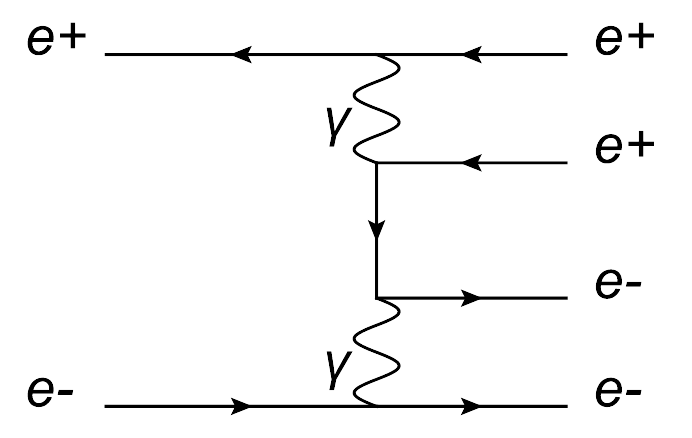
\includegraphics[height=5cm]{di-photon}
		\caption{major source of double photon QED background in Belle II }
	\end{figure}
	The beam background rate can be roughly regarded as the inverse square of radius from the IP. In the nano-beam scheme, the cutoff of beam interaction region is only about 10mm away from center. This is a good news for reconstruction of tracks and vertices but make the use of strip detectors in the first few layers impossible due to quite high occupancy, defined as the fraction of channels hit in every single triggered event.
	
	The concept of pixel followed by strip detectors has been proven successful by LHC. But not like the LHC experiment using rather thick silicon sensors as pixel material, the Belle II takes DEPFET (DEPleted Field Effect Transistor) technology as a option, because the low energy range of particles requires lesser equipped amplifiers electronics and cooling system to avoid too much multiple scattering in reconstructing vertices of B meson decay. 
	\begin{table}[hbp]
		\centering
		\caption{VXD Index, 1 and 2 are PXD, 3 to 6 are SVD}
		\huge
		\begin{tabular}{c|c|c|c|c|c|c}
			\hline
			Layer & 1 & 2 & 3 & 4 & 5 & 6 \\
			\hline
			Radius(mm) & 14 & 22 & 38 & 80 & 104 & 135 \\
			\hline
			Num of Ladders & 8 & 12 & 7 & 10 & 12 & 16 \\
			\hline
		\end{tabular}
	\end{table}
	\begin{figure}[htbp]
		\centering
		\includegraphics[height=7cm]{DEPFET}
		\caption{DEPFET and its silicon depleted structure}
	\end{figure}
	\begin{table}[hbp]
		\centering
		\caption{PXD geometry}
		\large
		\begin{tabular}{c|c|c|c|c}
			\hline
			Index & num of Ladders  & num of pixels & pixel size & sensitive region \\
				& $(mm)$ & ($z \times r\phi (\mu m^2)$) & ($z \times r\phi (mm^2)$)\\
			\hline
			Layer 1 & 8 & $768 \times 250$ & $55 \times 50 \ 60\times 50 $ & $44.8\times 12.5$\\
			\hline
			Layer 2 & 12 & $768 \times 250$ & $70 \times 50 \ 85\times 50 $ & $6.44\times 12.5$\\
			\hline
		\end{tabular}
	\end{table}
\section{Silicon Vertex Detectors}
	Working with the inner component PXD and outside Central Drift Chamber (CDC), SVD performs the measurement of two decay vertices in $B\text{-}\bar{B}$ mixing-induced CP violation through precise tracking and recontruction. In addition, SVD also serves for same purposes in D meson involved decay channels and $\tau$lepton decay. 
	
	SVD is designed with silicon sensors of strip channels along with two sides, vertical and parallel to the beam direction. This is for reducing a huge mount of readout channels using pixel detectors without compromising the vertex ability of Belle II.
	
	 The structure of Belle II can be illustrated as Fig 2-3. Since the SuperKEKB will collide the electron pairs at energy of 7 GeV and 4 GeV respectively, the Lorentz boost will be $\beta \gamma =0.28$, smaller than that of Belle. And this will lead a closer decay point of B mesons and its anti-particle. But considering the "Nano Beam Scheme" shrinks the interaction region of beam, this difference of B vertices is satisfying enough. 
	 \begin{figure}[htbp]
		\centering
		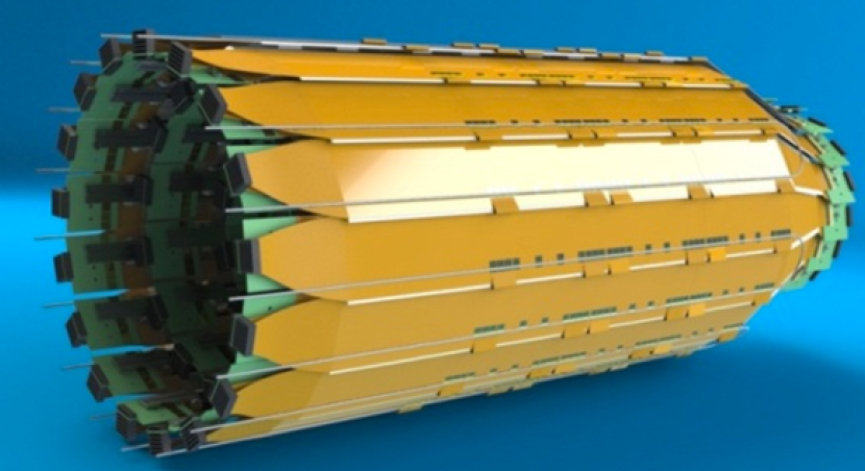
\includegraphics[height=7cm]{SVD}
		\caption{SVD structure with two side of hybrids readout and Origami flexible boards.}
	 \end{figure}
	
	\subsection{Requirements of SVD}
	The main characteristics of SVD in Belle II matches with the vertex environment quite well. The acceptance angle of SVD covers from $17^\circ \sim 150^\circ$, determined by the radius of PXD($38 mm$) and CDC($140mm$). By tracking the trace from outer detectors such as CDC and fitting with the pixels in PXD, the vertex reconstruction is done by SVD. 
	
	According to the experience of Belle and simualtion, the high occupancy should be assured lower about 10\% in order to get correct associated relationship between tracks reconstructed in CDC and hit combined in vertex detectors. Therefore, the proper two sides signals combination and geometry selection will be of much importance to eliminate combination background like ghost hit in SVD. 
	
	SVD must also apply its functions to low transverse momentum particles which will not hit out in CDC. And it must have enough reconstruction efficiency for those rather long life particles such as $K_{s}$ mesons. Since $K_s$ is a very important daughter particle in processes like $B\to K^{*}\gamma$ and $B\to K_s K_s K_s$ in which the only charged tracks come from $\pi$.
	
	Adequate stablity of SVD when facing perhaps 30 times higher event rate of Belle and up to 30kHz average trigger rate will determine the quality of data we collect from vertex detectors. To achieve this, SVD must be constructed with a fine design of high mechanical stablity and an efficient cooling system to dispense the power of heat. 
	
	SVD's associated software environment robustly maintains peak performance through ongoing and frequent calibrations, alignments, and monitoring.
	
	
	\subsection{SVD Layout}
	SVD is composed of 4 layers of "Double Sided  Silicon Detectors" ("DSSD"). The radius of these layers is listed as below:
	
	\begin{table}
		\large 
		\centering
	    \caption{SVD radius and readout chips numbers(128 channels per chip)},the most inner layer of SVD is indexed as "3" according to the scheme after the numbering of 2 PXD layers. 
		\begin{tabular}{c|c|c|c|c|c|c}
		\hline
		Layer & Radius & Ladders & Sensors/Ladder & Sensors & RO chips/sensor & RO chips \\
		\hline
		6 & 140 & 17 & 5 & 85 & 10 & 850 \\
		\hline
		5 & 115 & 14 & 4 & 56 & 10 & 560\\
		\hline
		4 & 80 & 10 & 3 & 30 & 10 & 300	\\
		\hline
		3 & 38 & 8 & 2 & 16 & 12 & 192 \\
		\hline
	    \end{tabular}
	\end{table}

 \begin{figure}[htbp]
	\centering
	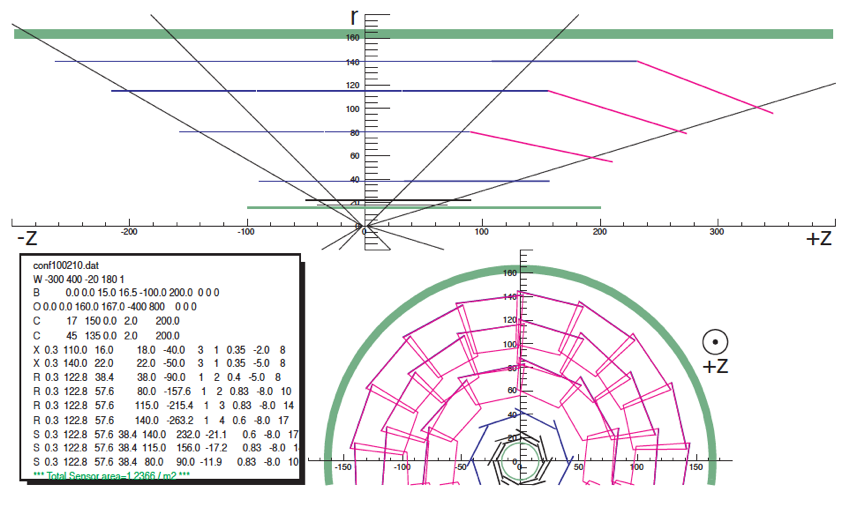
\includegraphics[height=10cm]{SVDgeo1}
	\caption{All SVD sensors (and PXD) configuration }
\end{figure}
	
	All DSSDs are located around the beam axis Z and have a overlapped area on the egde of them, which is called windmill design. P side of the sensors are parallel to and facing the Z axis. N side is facing towards the outside of detectors. The dimensions of sensors are demonstrated as Fig 2-5 and each of them are connected to APV25 chips.\cite{abe2010belle}
	
	\begin{figure}[htbp]
		\centering
		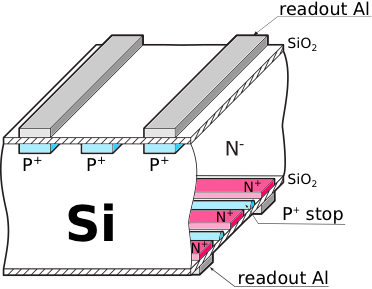
\includegraphics[height=7cm]{DSSD}
		\caption{DSSD silicon depleted structure}
		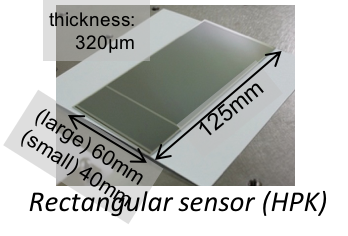
\includegraphics[height=5cm]{Rect}
		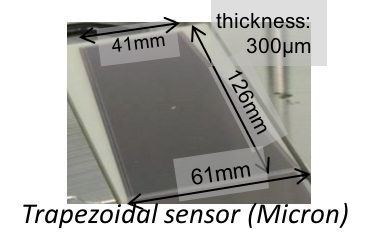
\includegraphics[height=5cm]{trap}
		\caption{Rectangular sensor (left) and Trapezoidal sensor (right) }
	\end{figure}

\subsection{APV25 readout and Origami design}
	To suppress the background hits, the fast readout chips with shaping time $\mathcal{O}(50 ns)$ are highly necessary and they have to be front-end, immune to rediation damage. In 2003, an assessment of readout ASICs was done, and the APV25 \cite{APV}, which was originally developed for the CMS silicon tracker, was chosen for the future vertex detector readout.
\begin{figure}[htbp]
	\centering
	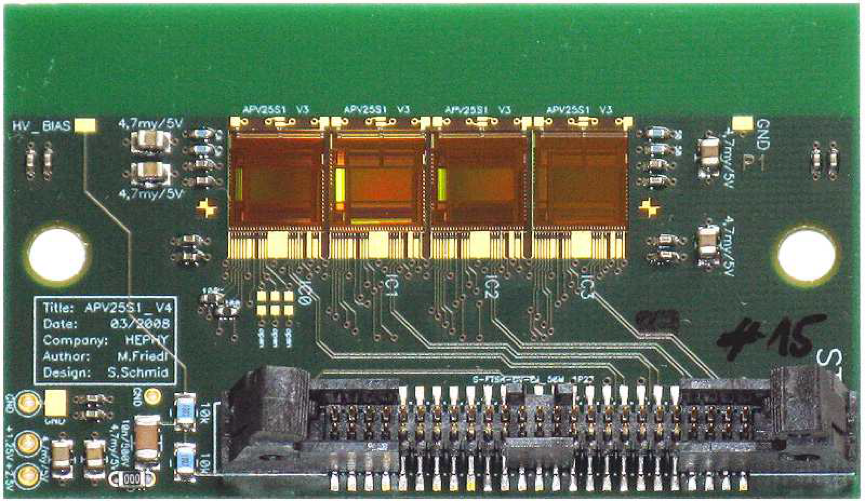
\includegraphics[height=8cm]{hybrid}
	\caption{APV25 chips on test PCB board}
\end{figure}

	\begin{figure}[htbp]
		\centering
		\includegraphics[height=7cm]{APV25}
		\caption{Block of one of 128 readout channels of APV25 front-end chip}
		
	\end{figure}


\begin{figure}[htbp]
	\centering
	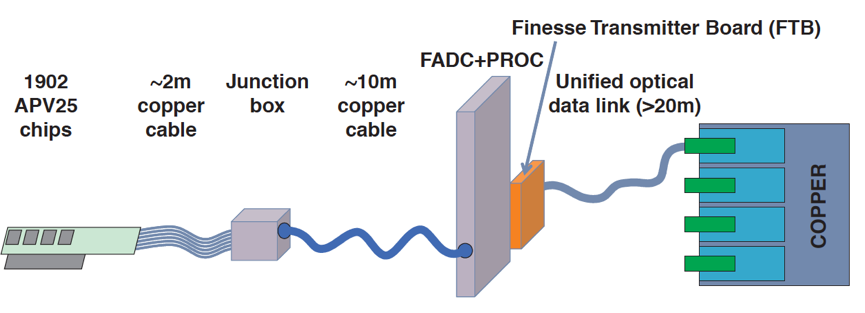
\includegraphics[height=6cm]{chain1}
	\caption{Schemetic view of SVD readout chain }
\end{figure}


	Except for the sensors that are located on the edge of acceptance and the inner layer 3, all the sensors are covered by the APV chips and readout system embeded structure called Origami which means "flexagon" in Japanese. This design is specialized for solving the issues that fast shaping time associated with higher susceptibility to noise. The capacitance distributed between the shaping modules and charge senstive preamplifier is the main course so the readout must be installed as close as possible to the amplifier. And that is where this "Chip-on-sensors" Origami concept comes in. Simply speaking, Origami design locates the APV25 chips on the cover of sensors with an airex layer between them, then the wire bonding operation performs wire bonding from the other side of sensors to the APV25 chips. In assembly of SVD ladders, the position accuracy of wire bonding and the gluing of covers of Origami is the key to the assurance of the quality of whole since the mismatch will not only affect the tolerance of ladder under an extreme environment close to IP but also directly affect the readout quality of SVD. If the origami is not proper wrapped bonding to the APV chips, the sensor can not transit any useful signal out and have to be replaced by new one.
	
	\begin{figure}[htbp]
		\centering
		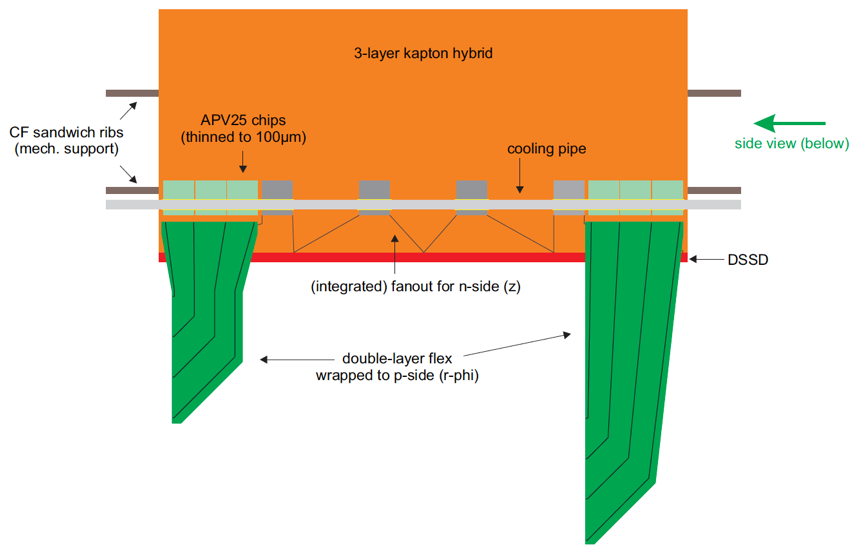
\includegraphics[height=8cm]{origami1}
		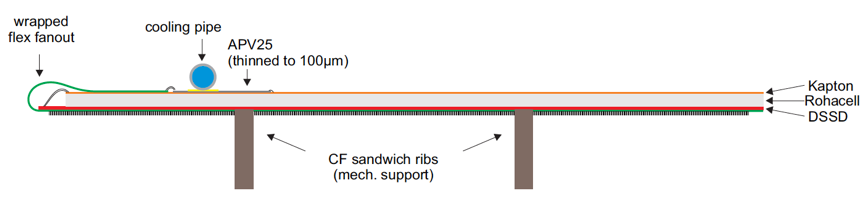
\includegraphics[height=4cm]{origami2}
		\caption{Top view and the side view of Origami with cover(orange) cooling pipe (gray) and wrapping belt (green)}. 
	\end{figure}

\begin{figure}[htbp]
	\centering
	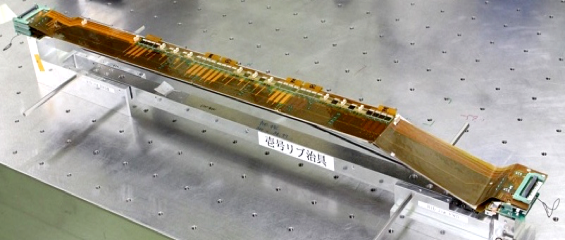
\includegraphics[height=6cm]{ladder}
	\caption{Single ladder of SVD on the assembly operating instrument  }
\end{figure}

\subsection{SVD assembly}
The overall structure of SVD consists of ladder's support, silicon sensors and electronics materials. Given the restrictive bugdet and the requirements of B Physics, the Origami concept, the sensors on the supporting ribs and end ring hybrid structure are designed. Two composite sandwich carbon fiber ribs (SCFR) are glued to the Origami sensor area in such a way that no structure interferes with the bond wires on the sensor side and shorts are avoided. To strengthen the stability of double end of electronics hybrid, another reinforcement of of ribs is attached with one layer of carbon fiber to have more stiffness in the joint area with the endring mount structure.

\begin{figure}[htbp]
	\centering
	\includegraphics[height=6cm]{endring}
	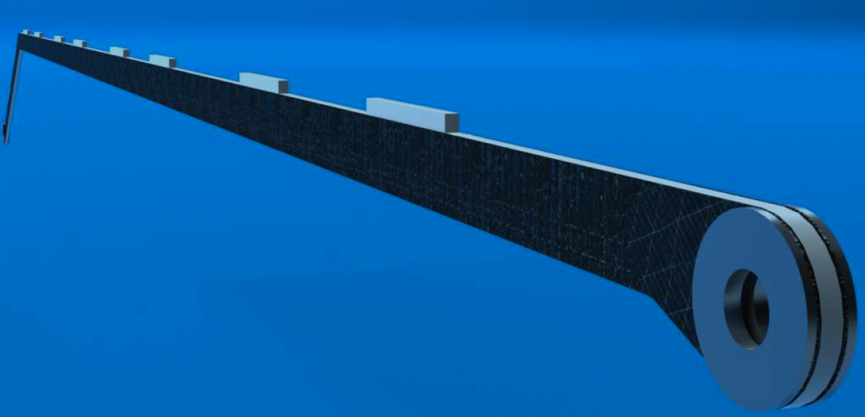
\includegraphics[height=4.7cm]{rib}
	\caption{Ladder of L6 scheme of sandwich composed rib (bottom) and endring mounts with hybrid board (top).}
\end{figure}

\begin{figure}[htbp]
	\centering
	\includegraphics[height=4cm]{endblock}
	\includegraphics[height=4cm]{elecboard}
	\caption{electronics hybrid board (right )and end mount supportor (left) of SVD L6}. 
\end{figure}

Since the hardware work I mainly participated is in the assembly of SVD L6, so the procedure of actual ladder assembly will be briefly described in the work of L6 group. Be awared of the difference of assembly between different layers, the detail can be varied. 

The whole assembly process is a finely designed, practically tested procedure that experienced many corrections and has been proven successful to meet the requirements mentioned before. The L6 ladder is composed of forward, backward, OCE (center),Z$\pm$ and Origami modules. And the general assembly procedure has following steps:

\begin{itemize}
	\item[-]Gluing of DSSD sensors with RA to the assembly bench which plays the role as a location lock and assembling platform in the whole process.
	\item[-]Placement of five DSSDs with alignment in a very high spatial precision, guranteed by the F mark (seal on the corner of each sensor) microscope check.
	\begin{figure}[htbp]
		\centering
		\includegraphics[height=4cm]{fmark}
		\caption{F mark on sensors' corner for position check}. 
		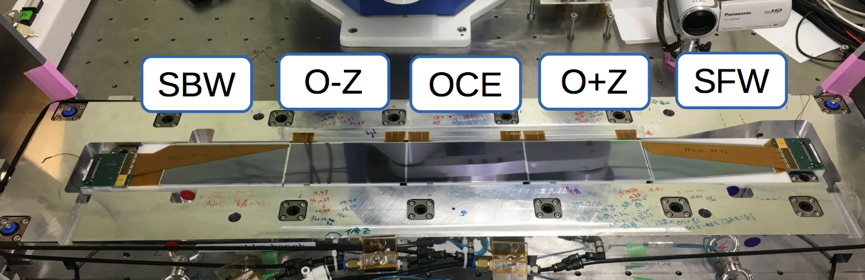
\includegraphics[height=4cm]{ladder3}
		\caption{Rough placement of DSSDs on assembly bench before the Origami gluing}
	\end{figure}
	\item[-] Backward and forward DSSDs are glued to rib with the pitch adapters and wire bond. OCE and Z$\pm$  (three modules) are glued to the Origami after the alignment.
	\item[-] Then the PA1 and PA2 at the corner of sensor will be wrapped to the other side of sensors and glued to the area of Origami where the APV25 channels are fan out prepared to bond with. 
	\item[-] Finally step is to combine the half ladder and the supporting structure (rib) and lock the screws.  
\end{itemize}

After the mechanical production of a ladder, the precsion check starts. First, the displacements of ladders on three directions are checked using CMM platform, which  assures the quality of mechanical performance. Then, taking advantage of the dark box in the clean room and data aquisition system, the electronic performance of ladder can testified. When a ladder passes the quality check, it will be carefully packed and stored in the shelter for further use. For those that can not be used in real experiment or beam test, they will be either abandoned or kept for assembly procedure validation purposes based on to what extend they are damaged or deformed. 

\begin{figure}[htbp]
	\centering
	\includegraphics[height=6cm]{CMM}
	\caption{CMM measurement platform}
	\space 
	\includegraphics[height=4cm]{daq1}
	\includegraphics[height=4cm]{daq2}
	\caption{Chamber for electronics and source test(left),Data Aquisition computers(right)}
\end{figure}

The detailed assembly procedures including common assembly, Origami Modules assembly, gluing and wire bonding are not the main body here. Since Spring of 2016, after several runs of assemly procedures study and practice, massive production of SVD L6 was offically started. By April of 2017, nine ladders of L6 have been manufactured and four passes the quality assurance that allows them to be used in real experiment. The first ladder was shipped to DESY, Germany for 2016 and 2017 beam test. In future, there will be 20 working ladders for L6. Approximately, one ladder assembly and test takes up for 15 days, so by the end of Nov. of 2018, the whole massive production of SVD shall be finished if no more expected issues occurs. 

\begin{figure}[htbp]
	\centering
	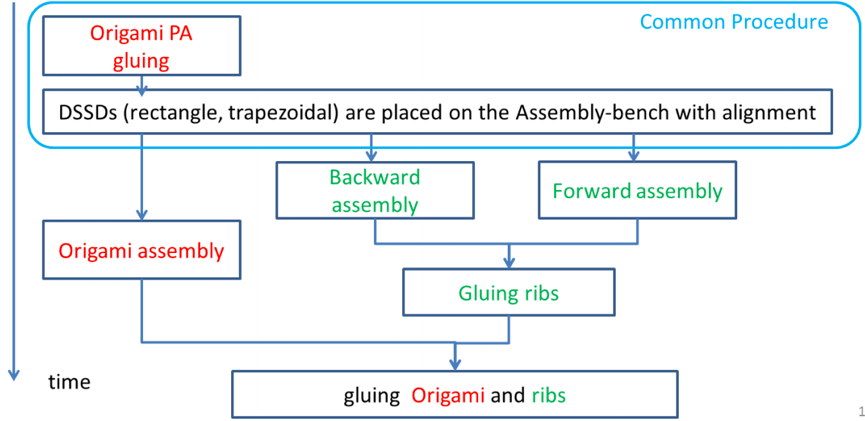
\includegraphics[height=6cm]{step1}
	\caption{Timing of assembly of SVD L6 procedures\cite{shimizu}}. 
	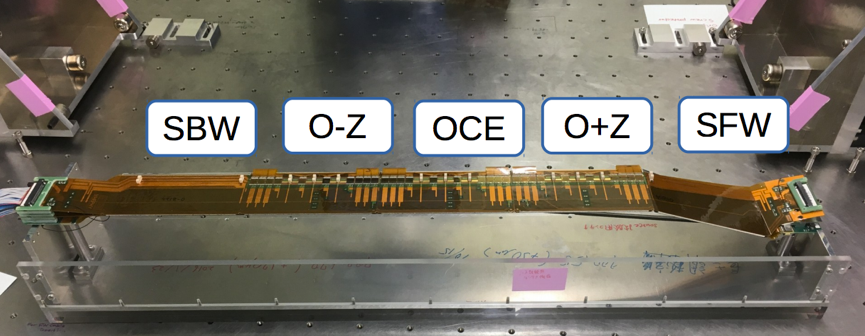
\includegraphics[height=6cm]{ladder2}
	\caption{Finished ladder of L6}
\end{figure}

\section{Ghost hits reduction}
	To meet the vertexing environment of Belle II, SVD has been designed and produced as a set of multi-layers double sided strip detectors. Like we introduced in the section 2.2.1, the occupancy has to be controlled in lower 10\% and need to be optimized as low as possible in order to find proper tracks with outer detectors. 
	However, the feature of SuperKEKB creates average 30kHz environment and it benefits the physics with a high statisitical accuracy, which make sacrificing this high luminosity to meet the occupancy requirments the loss that outweights the gain. This leads a desire to reduce the background through software side, such as finding proper variables to distinguish the physical hit from an interested particle rather a background. 
	
	\begin{figure}[htbp]
		\centering
		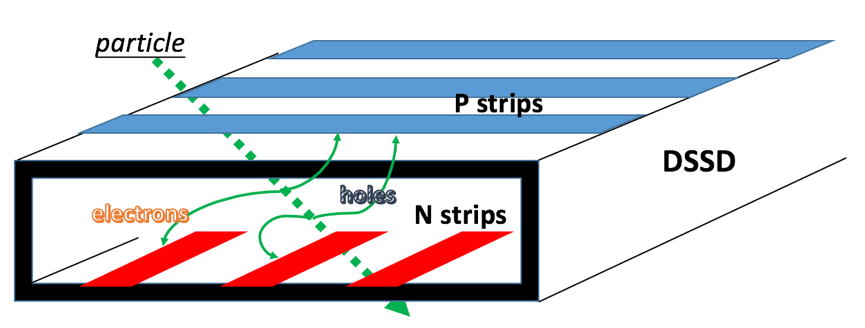
\includegraphics[height=6cm]{svdhit}
		\caption{illustrative process of particle depositing energy in SVD depleted area and create two side signal correspondingly.}. 
	\end{figure}
	
	Especially in one SVD event, two side of strips read-out channels can cause combinational background from wrongly associating two-side hit from two particles or electronical noise into one (see Fig 2-20), and it's named "ghost hits" since they are completely programmed background and has no physics process related to. The work of tracking can surely eliminate most of these ghost hits since only the ones who close enough to real hits will make trouble to tracking, but still,  the rest of them is a concern from Belle experience and simulation. It mainly refers to the occupancy on layer 3 of SVD due to its close location to the interaction region. The event rate can be roughlt regarded as inverse-square of the radius which is psoitively approved by the latest MC Campaign.
	
	\begin{figure}[htbp]
		\centering
		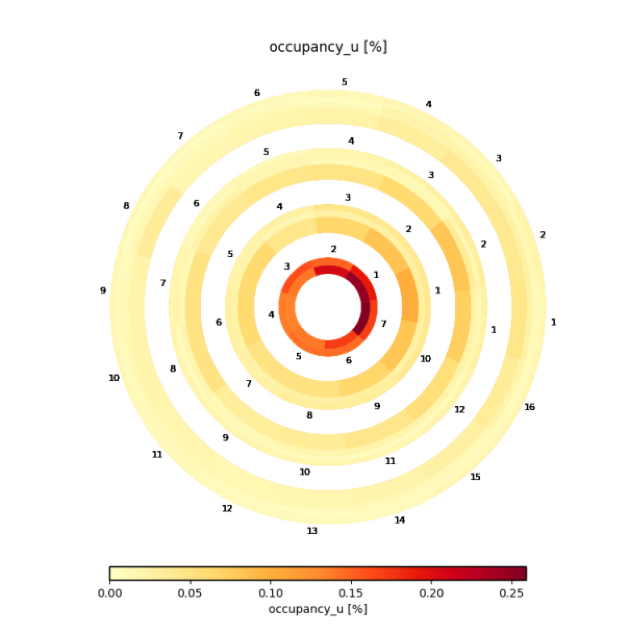
\includegraphics[height=7cm]{svdocc}
		\caption{P side of SVD occupancy from simulation compaign 12\&15, by Peter Kvasnicka, May 2017}
	\end{figure}
	
	Moreover, tracking in Belle II is based on the hit, which is a spacepoint independent from detectors, input to the data handling path. Tracking is one of the most time consuming process of online data tracking and it is crucial to the high level trigger (HLT) by offering the selection of region of interests in PXD sensors to cut off useless signals. This raise a need for fast tracking speed and apparently, lossing such time on fitting the track where ghost hits locates isn't a wise choice, not mention that there is a limited requirement in data taking speed on readout bandwidth for PXD and SVD, see Tab 2.5. Then, the effective ghost hits reduction on software is rather important to save the computational resources, which in general it's where this thesis stands for. 
	
	
\begin{figure}[htbp]
	\centering
	\includegraphics[height=10cm]{ghosthit}
	\caption{illustrative scheme for ghost hits, similar color means readout from a true hit, and wrong combination happens when two or more hits are recorded in one event.}
\end{figure}

\begin{table}[htbp]
	\large
	\centering
	\begin{tabular}{c|c|c|c|c|c}
		\hline
		- & \#ch & occ & ch size & evt size & total \\
		- & - & \% & bit & bit & bit\\
		\hline
		PXD & 8M & 1 & 4 & 320k & 7.2G \\
		SVD & 24k & 1.9 & 4 & 18.5k & 555M \\
		\hline
	\end{tabular}
	\caption{Estimated average occupancy and data size and required number of subcomponents\cite{abe2010belle}, ch and occ stands for channel and occupancy respectively.}
\end{table}

Driven by this demand, we would like to take other information excluding location of hits into account to reject ghost hits, such as the charge deposition and timing infomation. Charge deposition from one particle can be regarded similar on both side of SVD sensors rather these from different particles are not, or least not has to be. 
The potential deviation of charge deposition could be used effectivly to distinguish ghost hits. Of course, timing information maybe more straightforward to this idea and probably more sensitive but due to the online timing tag and calibration imperfection, we shall cut in through the charge information and design our analysis tools in a flexaible way, perhaps for further utilizing timing information. To fullfill this idea and realize the significance of the thesis, a comprehensive understanding of Belle II software structure and function becomes a must particularly in tracking part. Following chapters will start from the introduction Belle II software, leading a way to the realization of ghost hits reduction feasiblilty study using test beam data sequentially. 



